\documentclass[conference]{IEEEtran}
\usepackage{cite}
\usepackage{graphicx}
\usepackage{booktabs}
\usepackage{amsmath,amssymb}
\usepackage{url}

\newcommand{\tierm}{\textsc{measured}}


\begin{document}

\title{Symbolic Feature-Basis Adequacy Certification\\
for Game Value Compression: A Z3 Case Study}

\author{\IEEEauthorblockN{mikeewwwwwwwwww}
\IEEEauthorblockA{Independent Research\\
mikeewwwwwwwwww@users.noreply.github.com}}

\maketitle

\begin{abstract}
Compiling an exact game value function into a multi-terminal binary decision
diagram (MTBDD) over semantic features is sound only if the feature basis is
\emph{value-sufficient}: two states with equal feature vectors must have
equal values. We formalize this adequacy condition as an existential SMT
query and certify it with Z3 for a family of solved chess-fragment classes
(kings, pawns, and knights on $N\times N$ boards, up to 1.36M states per
class). The v1 feature basis of the underlying pipeline is refuted on all
seven classes---with concrete, machine-checked counterexamples on the six
classes that publish pairs, the mirror-symmetric class being certified by
the VAL-free symmetry proof of \S\ref{sec:mirror} instead---exhibiting
three distinct ambiguity mechanisms: knight-square geometry, rank
translation, and pawn geometry. The repaired v2 basis---signed per-axis
piece-to-king offsets, king rank-edge distances, and signed pawn
offsets---closes all seven classes: one full-class unsat proof, five
bounded-subspace unsat proofs, and one perfect-injectivity empirical layer
above the array-axiomatisation budget. A separate VAL-free proof establishes
that the feature map commutes with the colour-swap mirror (unsat in
0.25\,s), and 136{,}068 cross-oracle evaluations agree exactly. The
methodological contribution is a budgeted adequacy certificate: cheap to
run, refutation-first, and honest about which classes carry full proofs,
subspace proofs, or empirical evidence only.
\end{abstract}

\begin{IEEEkeywords}
SMT solving, Z3, decision diagrams, game solving, feature engineering,
verification, chess endgames
\end{IEEEkeywords}

\section{Introduction}
When a solved game's value function is compiled into a compressed evaluator,
the compiler makes an invisible assumption: that the features it tests carry
\emph{all} the information the values depend on. If two states share a
feature vector but differ in value, the compiled structure must either
encode extra coordinates (a ``tail'') or it silently mis-evaluates. In the
K2P compression pipeline \cite{k2p2025}---a solved $4\times4$ chess fragment
whose value function is compiled into zero-lookup MTBDD evaluators---this
assumption was initially trusted on empirical evidence alone (zero observed
conflicts). That evidence was insufficient: when the pipeline was extended
to knight-bearing material (K2P+N), a symbolic check found the assumption
false on every class tested, with certified counterexamples that directly
drove the repair.

This paper is a case study in turning that assumption into a certificate.
We formalize feature-basis adequacy as an existential SMT query over the
class's state space, encode states, legality, features, and values in Z3
\cite{demoura2008,demoura2011}, and run a refutation-first protocol: try to
break the basis; if it breaks, extract and certify counterexamples; if it
survives, prove it---fully when the array axiomatisation fits the budget,
otherwise on a bounded subspace, with the empirical layer covering the rest.
The protocol closed on a chess-fragment family of seven material classes
(2{,}112 to 1{,}358{,}808 states), produced a minimality ladder showing
which feature families are load-bearing, and yielded a VAL-free mirror
symmetry proof. The companion scaling paper \cite{ccs2026} reports the
compression measurements this certification underwrites.

There is an order-of-trust question here as well as a measurement one.
Empirical validation---enumerate every state, evaluate, compare---is cheap,
complete for correctness, and silent in the best sense: it either finds a
mismatch or it does not. But it cannot say \emph{why} a representation
works, it cannot be consulted when the representation is extended to new
material, and its clean verdict on an old family says nothing about a new
one. A symbolic certificate reverses the order: it fails fast and loud
(concrete witnesses), or it proves the property outright, and its cost is
bounded by explicit budgets rather than by trust. The protocol in this
paper is built around that reversal, and its per-class verdicts record
exactly how far the certificate reached on each class.

The contributions are:
\begin{itemize}
\item a formal statement of feature-basis adequacy for feature-based
MTBDD compilation (\S\ref{sec:problem}) and a Z3 encoding of states,
legality, features, and values that supports both refutation and proof
(\S\ref{sec:encoding});
\item a refutation of the v1 basis on all seven classes, with three
certified ambiguity mechanisms and a decoded counterexample pair
(\S\ref{sec:v1}, Fig.~\ref{fig:counter});
\item the v2 repair (signed offsets + rank-edge distances + signed pawn
offsets), a minimality ladder over feature subsets, and closure on all
seven classes with per-class proof tiers (\S\ref{sec:v2},
Tables~\ref{tab:v1}--\ref{tab:status});
\item a VAL-free mirror-symmetry proof and a 136{,}068-agreement
cross-oracle check (\S\ref{sec:mirror}); and
\item an explicit account of what the certificate proves and what it does
not (\S\ref{sec:limits}).
\end{itemize}

\section{Problem Statement}
\label{sec:problem}

\subsection{Value functions over finite game graphs}
Let $G=(S,E)$ be the game graph of a finite, perfect-information,
two-player game under a fixed ruleset, with $S$ the set of legal
states (a state includes the side to move). The retrograde oracle computes
the mover-relative value $\mathrm{VAL}: S \to \{\mathrm{win}, \mathrm{loss},
\mathrm{draw}\}$ exactly---including the cycle-draw convention for
unresolvable repetitions---by backward induction over $E$
\cite{thompson1986,allis1994}. Databases of this kind are the classical
substrate of endgame solving \cite{nalimov2000,schaeffer2007,vanherik2002};
the contribution here is not the oracle but the certificate attached to its
compressed representation. Two conventions matter for everything that
follows. First, values are \emph{mover-relative}: VAL(s) is the result for
the player to move at s, which halves the state space relative to a
white-to-move convention and makes mirror symmetry a value-preserving map
rather than a value-negating one. Second, unresolvable repetition cycles
are decided as draws by a fixed-point convention (cycle draws), so VAL is
total over legal states and the array axiomatisation of
\S\ref{sec:encoding} is exact rather than partial.

\subsection{MTBDD as compressed evaluator}
The compiler groups states by a symmetry quotient (colour swap and board
reflection), assigns each orbit a semantic feature vector
$\varphi(s) \in \mathbb{Z}^d$ (relative distances, alignments, attack and
check counts, material counts, tempo), and builds an ordered MTBDD
\cite{bryant1986,bryant1992,bahar1997,fujita1997,burch1992} over the
features, with a conditional coordinate tail appended when features alone
cannot separate value classes. The construction is deterministic: orbits
are sorted, rows are sorted lexicographically over the feature vector, and
the MTBDD is built over the features in a fixed order (with the tail
coordinates tested after the semantic features, only on the rows that
need them). The emitted evaluator is a pure-integer
branching program: no tables, no arrays, no search on the evaluation path.
Its correctness criterion is exact agreement with $\mathrm{VAL}$ on every
legal state, which the pipeline checks exhaustively at these scales (all
6{,}744{,}724 states at $N{=}5$; every class run in the underlying study
verified with zero mismatches).

\subsection{The injectivity question}
Grouping states by feature vector is sound iff the basis is
\emph{value-sufficient} on the class $C$:
\begin{equation}
\forall s_1, s_2 \in C:\ \varphi(s_1) = \varphi(s_2) \Rightarrow
\mathrm{VAL}(s_1) = \mathrm{VAL}(s_2).
\label{eq:inj}
\end{equation}
Note the direction: (\ref{eq:inj}) is a \emph{sufficient} condition for
correct compilation without a tail, not a necessary one (the tail restores
correctness regardless), and it makes no claim about compression ratio.
Empirically, (\ref{eq:inj}) can only be verified by enumerating all
$|C|^2$ pairs---or, better, by observing that equal feature vectors define
equivalence classes whose value sets must be singletons, which is
checkable in $O(|C|)$ bucketing. But the empirical check says nothing
about \emph{why} the basis works or how to repair it when it fails, and it
cannot distinguish a sound basis from an unlucky sample. The symbolic
query answers both: it certifies refutation with a concrete pair when
(\ref{eq:inj}) fails, and proves it when it holds.

\section{Z3 Encoding}
\label{sec:encoding}

\subsection{State space and legality}
Each class fixes a material vector (per side: king always; pawn and/or
knight flags) and a board size $N$. A state is packed into seven 16-bit
fields $[\mathrm{wk}, \mathrm{bk}, \mathrm{wp}, \mathrm{bp}, \mathrm{nw},
\mathrm{nb}, \mathrm{stm}]$ (square index $x + yN$; absent pieces fixed to
the sentinel $-1$; $\mathrm{stm} \in \{0,1\}$). Sixteen bits are enough to
hold any square index, the sentinel, and the sign bit for signed
intermediate values, which keeps the bit-blasted arithmetic small. In Z3,
two fresh symbolic states $s_1, s_2$ are created as BitVec variables of
width 16 per field; absent-piece fields become the constant sentinel, so
the solver never explores material configurations outside the class. The
legality predicate is rewritten symbolically from the solver's own
rules (kings never adjacent; pawns blocked by occupancy and captured
diagonally; promotion constrained by board edge; knight moves and captures;
the side \emph{not} to move may not be in check; no illegal sentinels), so
that $\mathrm{legal}(s)$ characterises exactly the class's legal states.
A bijective packing $\mathrm{ENC}(s)$ into 32 bits---a mixed-radix product
of the per-piece indices and the tempo---makes every legal state a distinct
array key, which is what allows the value oracle to enter the encoding as
an array lookup rather than a per-state predicate.

\subsection{Feature extraction}
The feature map $\varphi$ is re-implemented over the BitVec fields with the
\emph{same feature names and definitions} as the compression pipeline's
Python implementation: modular per-axis differences (wrap-around arithmetic
with modulus $N^2{+}1$ handles board-edge distances), Chebyshev distances as
$\max$/$\min$ of absolute modular deltas, knight-attack and check counts,
alignment features, rank-edge distances, and the v2 signed offsets
(\S\ref{sec:v2}). Unsigned division and remainder by $N$ extract file and
rank; signed interpretations are applied after the fact so that the
bit-blasted arithmetic matches the Python semantics exactly, including the
sentinel propagation (any feature involving an absent piece is the
sentinel, not a computed value). Each v1 counterexample check and each
proof run is accompanied by unit self-tests that evaluate the symbolic
$\varphi$ on 500 concrete states per class and compare against the Python
extraction, exactly; an encoding that drifts from the pipeline's features
would fail these tests (and, in the other direction, a \textsc{sat} result
where the empirical layer reports zero conflicts is flagged as a suspected
encoding bug and reported as such).

\subsection{The injectivity query and the value oracle}
The value function enters the encoding as an SMT array
$\mathrm{VAL} : \mathsf{BV32} \to \mathsf{BV8}$, constructed as a chain of
$\mathsf{Store}$ operations---one per class state---at the packed encodings
with the oracle's values. The array is therefore an exact finite map of the
class, and the query
\begin{equation}
\begin{aligned}
\exists s_1 s_2:\ &\mathrm{legal}(s_1) \wedge \mathrm{legal}(s_2) \wedge
\varphi(s_1) = \varphi(s_2)\\
&\wedge\ \mathrm{VAL}[\mathrm{ENC}(s_1)] \neq \mathrm{VAL}[\mathrm{ENC}(s_2)]
\end{aligned}
\label{eq:query}
\end{equation}
ranges over exactly the class. Because the array must enumerate one
$\mathsf{Store}$ per state, the axiomatisation has a hard budget
(\texttt{--max-proof-states}, 60{,}000 in this study): classes above the
cap cannot carry a full proof, whatever their size. The remaining protocol
budgets are equally explicit: 300\,s per full-class or subspace proof, a
subspace target of 10\% of the class, and a cap of 12 certified
counterexample pairs per class (one per reported bucket, up to the cap).
The protocol per class
is (Fig.~\ref{fig:pipeline}):
\begin{enumerate}
\item \textbf{empirical layer}: bucket all $|C|$ states by feature vector
in Python; record conflict buckets;
\item \textbf{if conflicts exist}: extract one pair per bucket, re-verify
each pair \emph{symbolically} (both states concrete, both legality and
feature equality re-encoded in Z3), and report \textsc{refuted} with
machine-checked counterexamples;
\item \textbf{if no conflicts}: attempt the full-class query
(\ref{eq:query}); \textsc{unsat} $\Rightarrow$ \textsc{proved}; timeout
$\Rightarrow$ fall through;
\item \textbf{subspace proof}: restrict to a geometric subspace (white king
square $< K$, with $K$ grown until the subspace covers $\ge 10\%$ of the
class or hits the array cap); \textsc{unsat} there $\Rightarrow$
\textsc{proved\_on\_subspace};
\item \textbf{otherwise}: \textsc{empirical\_only}.
\end{enumerate}

\begin{table}[t]
\caption{Protocol parameters (command-line defaults of the committed
script; Z3 5.4.1).}
\label{tab:params}
\centering
\footnotesize
\setlength{\tabcolsep}{3pt}
\begin{tabular}{ll}
\toprule
bit-vector width per field & 16 \\
state packing width & 32 bits (bijective) \\
full-class / subspace proof budget & 300\,s each \\
array axiomatisation cap & 60{,}000 states \\
subspace target & 10\% of class ($wk{<}K$) \\
counterexample certification cap & 12 pairs \\
$\varphi$ self-test & 500 states, exact \\
\bottomrule
\end{tabular}
\end{table}

The cost profile is asymmetric, and deliberately so. The empirical layer is
$O(|C| \cdot d)$ hashing---seconds for every class in this study, including
the 1.36M-state class---and it runs first because it is where most defects
are caught. The symbolic layer's cost is dominated by bit-blasting the
feature arithmetic and by the array construction: proof time grows with
the axiomatised state count (1.7\,s for 2{,}112 states to 22.8\,s for
22{,}375), and the two full-class attempts that exhausted their budgets
returned \emph{unknown} rather than a wrong answer, which is the failure
mode the tier system is designed to absorb.

\begin{figure}[t]
\centering
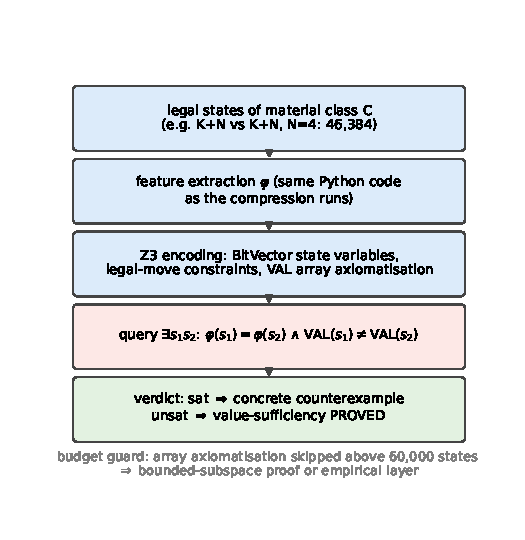
\includegraphics[width=\columnwidth]{figures/f1_pipeline.pdf}
\caption{The certification pipeline. The empirical layer is the fast
refutation path; the symbolic layer certifies. Budgets are explicit, and
the verdict records which tier was reached.}
\label{fig:pipeline}
\end{figure}

\subsection{Why the empirical layer was not enough}
The empirical layer of this protocol---bucket all states by feature vector
and check that every bucket's value set is a singleton---is exactly the
check the underlying pipeline had been running informally all along, and on
the knight-free families it had always come back clean: the committed
family builds report zero semantic conflicts on canonical rows, and the
coordinate tail was never needed. The knight extension broke that record
immediately, and it broke it on classes whose empirical behaviour looked
benign at small scale (the K+N vs K+N classes have only 4--6 conflict
buckets out of thousands of vectors). The lesson is not that the empirical
layer is worthless---it catches the vast majority of defects and is the
fast refutation path here---but that it cannot distinguish ``the basis is
sound'' from ``no counterexample happened to be enumerated yet'', and it
offers no help at all when the question becomes \emph{which} feature is
missing. The symbolic layer answers both: it turns ``0 conflicts observed''
into a proof where the basis is sound, and its counterexamples into a
diagnosis where it is not.

\section{v1 Refutation}
\label{sec:v1}

\subsection{The query is sat for every class}
Basis v1---the basis of every committed compression run of the underlying
pipeline---consists of 5 king features (tempo, king distance, opposition
orientation, edge distances) and 13 knight features (counts, distances,
attack/check and capture relations), extended by 14 pawn features on pawn
classes: 18 features on knight-only classes, 32 on pawn classes. The query
(\ref{eq:query}) is \textsc{sat} on all seven classes: 4 to 17{,}892
conflict buckets per class (Table~\ref{tab:v1}). Every published bucket
pair was re-verified symbolically, so the counterexamples are not empirical
accidents but certified members of the class; the mirror class publishes
no pair---its v1 record is empirical conflict buckets only (2{,}946), and
its dedicated certification is the mirror-symmetry proof and the
136{,}068-agreement cross-oracle check of \S\ref{sec:mirror}, hence the
``--'' in the certified column. The symbolic re-verification
matters because the buckets are found by Python hashing: a bucketing bug
would produce phantom pairs, and re-encoding both states from scratch in
Z3---legality, features, and values independent of the bucketing code---rules
that out before the refutation is published.

\begin{table}[t]
\caption{v1 refutation per class (\tierm{};
z3\_injectivity.json). States = legal class states; conflicts = feature-equal
buckets with differing oracle values; certified = machine-checked
counterexample pairs; $\varphi$-distinct = distinct feature vectors.}
\label{tab:v1}
\centering
\footnotesize
\setlength{\tabcolsep}{3.2pt}
\begin{tabular}{lrrrrr}
\toprule
class & $N$ & states & $\varphi$-distinct & conflicts & certified \\
\midrule
kn     & 3 & 2{,}112 & 290 & 4 & 4 \\
kn     & 4 & 46{,}384 & 6{,}328 & 6 & 6 \\
kn     & 5 & 391{,}072 & 55{,}312 & 6 & 6 \\
kpn    & 4 & 25{,}178 & 5{,}469 & 518 & 12 \\
kpn    & 5 & 249{,}728 & 39{,}307 & 4{,}004 & 12 \\
mirror & 4 & 136{,}068 & 43{,}489 & 2{,}946 & -- \\
both   & 4 & 1{,}358{,}808 & 568{,}978 & 17{,}892 & 12 \\
\bottomrule
\end{tabular}
\end{table}

\subsection{Counterexample anatomy}
Three mechanisms account for all certified counterexamples.
\textbf{(1) Knight-square ambiguity} (dominant): positions differing only
in the knight's exact square can share every distance feature---Chebyshev
norms deliberately discard direction---yet differ in mate-net geometry, and
hence in value. Fig.~\ref{fig:counter} decodes one certified pair from the
K+N vs K+N, $N{=}4$ class: with white king a1, white knight a2 and black
king c2, the black knight on d2 yields a mover win, the black knight on d3
a draw; all 18 v1 features are identical (the pair shares a bucket of size
28). The mate that works through d2 fails through d3 because the
\emph{direction} of the knight's relation to both kings changes while every
symmetric distance stays put.
\textbf{(2) Rank-translation ambiguity}: whole positions shifted along the
rank axis preserve every signed relative geometry---signed deltas are
translation-invariant too---but edge-dependent mates depend on the absolute
rank band; only an edge-distance feature can pin it. The certified pair
$[0,6,-1,-1,4,2,1]$ (mover wins) versus $[4,10,-1,-1,8,14,1]$ (draw),
bucket size 12, is this mechanism made concrete: the entire position
(white king a1, black king c2, white knight a2, black knight c1) is
translated one rank away from the bottom edge (to a2, c3, a3, c4), every
relative feature including the knight-to-king Chebyshev distance (2) is
unchanged, and the value flips from win to draw because the mating geometry
that depends on the rank-1 edge has been destroyed.
\textbf{(3) Pawn-geometry ambiguity} (pawn classes): pawn placements at the
same distances from both kings and the knight but on different files carry
different promotion races and capture geometries. These mechanisms are not
independent pathologies: they all instantiate the same principle---a basis
of undirected and translation-invariant features cannot distinguish
configurations that differ only in orientation or edge proximity, exactly
the configurations chess endgames care about.

\begin{figure}[t]
\centering
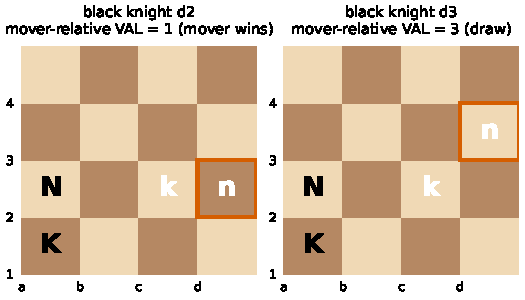
\includegraphics[width=\columnwidth]{figures/f2_counterexample.pdf}
\caption{A certified v1 counterexample pair (K+N vs K+N, $N{=}4$;
states $[\mathrm{wk},\mathrm{bk},\mathrm{wp},\mathrm{bp},\mathrm{nw},
\mathrm{nb},\mathrm{stm}]$, squares indexed $x+y\cdot4$):
$s_1 = [0,6,-1,-1,4,7,1]$ (knight d2), mover-relative
$\mathrm{VAL}=1$ (mover wins); $s_2 = [0,6,-1,-1,4,11,1]$ (knight d3),
$\mathrm{VAL}=3$ (draw). All 18 v1 features are equal
(bucket size 28); the difference is pure mate-net geometry.}
\label{fig:counter}
\end{figure}
\section{v2 Fix}
\label{sec:v2}

\subsection{Signed knight offsets, rank-edge distances, pawn offsets}
The mechanisms of \S\ref{sec:v1} dictate the repair. Against knight-square
ambiguity, the basis needs the knight's \emph{direction}, not just its
distance: basis v2 adds eight signed per-axis offsets, four per colour
($k\_dx_w, k\_dy_w$: white knight to white king; $k\_dxe_w, k\_dye_w$:
white knight to black king; and the black counterparts), each defined as
the signed per-axis delta $\mathrm{king} - \mathrm{piece}$ with sentinel
$-1,-1$ when the piece is absent. Against rank-translation ambiguity, the
basis needs an absolute-rank anchor: v2 adds two king rank-edge distances
$re_w, re_b = \min(y, N{-}1{-}y)$. Against pawn-geometry ambiguity, v2
adds eight signed pawn offsets (pawn to own king, pawn to enemy king, per
axis). The result is 28 features on knight-only classes and 50 on pawn
classes. The v1 API of the underlying basis module is unchanged, so every
previously committed compression run remains reproducible; the v2 features
are an addition, tested by the same certification protocol.

\subsection{Minimality ladder}
Signed knight offsets alone were the \emph{naive} fix hypothesis, and the
ladder refutes it: subsets $\{A\}$, $\{B\}$, and $\{A,B\}$ (own, enemy,
both signed knight-offset families) close \emph{no} class---they leave 4 to
16 conflict buckets on the knight classes and 441 to 8{,}192 on the pawn
classes (Table~\ref{tab:ladder}). The certified closure combinations are:
knight-only classes close with one signed family \emph{plus} the rank-edge
pair ($\{A,C\} = \{B,C\} = 0$ at every $N$; $\{A,B\}$ without $C$ keeps 8
buckets, so $C$ is required there); pawn classes close with both signed
knight families plus signed pawn offsets ($\{A,B,D\} = \{A,B,E\} = 0$),
where the rank-edge pair is redundant. An opponent-orientation split $O$
(same-file vs.\ same-rank alignment) changes nothing on any class and was
dropped. The shipped v2 basis $\{A,B,C,D,E\}$ is therefore mildly
overdetermined by design---one class-independent definition rather than
per-class minimality---which is a deliberate trade: a single basis across
classes keeps the pipeline uniform, at the cost of two redundant feature
families per class type.

\begin{table}[t]
\caption{Minimality ladder: conflict buckets under feature subsets
(\tierm{}; minimality\_ladder in z3\_injectivity\_v2.json). Shorthand: kn =
K+N vs K+N; kpn = K+P+N vs K; mirror = K+P vs K+P+N; both = K+P+N vs
K+P+N. A = knight$\to$own signed offsets; B = knight$\to$enemy;
C = king rank-edge distances; D = pawn$\to$own signed offsets;
E = pawn$\to$enemy; O = opp-orientation split (redundant everywhere,
dropped). Bold 0 = closed.}
\label{tab:ladder}
\centering
\footnotesize
\setlength{\tabcolsep}{3pt}
\begin{tabular}{lrrrrrrr}
\toprule
class & v1 & A & B & AB & AB+C & AB+D & AB+E \\
\midrule
kn, $N{=}3$ & 4 & 4 & 4 & 8 & \textbf{0} & -- & -- \\
kn, $N{=}4$ & 6 & 8 & 8 & 8 & \textbf{0} & -- & -- \\
kn, $N{=}5$ & 6 & 16 & 8 & 8 & \textbf{0} & -- & -- \\
kpn, $N{=}4$ & 518 & 774 & 538 & 441 & -- & \textbf{0} & \textbf{0} \\
kpn, $N{=}5$ & 4{,}004 & 8{,}192 & 6{,}305 & 6{,}932 & -- & \textbf{0} & \textbf{0} \\
mirror, $N{=}4$ & 2{,}946 & 3{,}186 & 3{,}202 & 2{,}097 & -- & \textbf{0} & \textbf{0} \\
both, $N{=}4$ & 17{,}892 & 7{,}674 & 8{,}054 & 7{,}400 & -- & \textbf{0} & \textbf{0} \\
\bottomrule
\end{tabular}
\end{table}

\subsection{Result: all classes close}
Under basis v2 the query (\ref{eq:query}) is \textsc{unsat} on all seven
classes: zero conflict buckets, with the empirical layer simultaneously
perfect or near-perfect (the knight classes retain a largest bucket of 2:
96 class states at $N{=}4$ and 576 at $N{=}5$ share a feature vector with
exactly one other state, and the oracle evaluates both identically; the
pawn classes reach exact injectivity on the two
largest classes, 1{,}358{,}808 states mapping to 1{,}358{,}808 distinct
vectors). Table~\ref{tab:v2} gives the aggregate; Table~\ref{tab:status}
gives the per-class proof tier and timing. The proof tiers differ for
budget reasons only (\S\ref{sec:limits}); the empirical layer is clean on
the full class in every case.

Two scope notes keep this result honest. First, the near-buckets on the
knight classes mean v2 is value-sufficient but not perfectly injective as a
map: two states may still share a feature vector, but when they do, they
agree in value, which is exactly the property compilation needs. Second,
the compression runs of the underlying study were compiled with the v1
basis plus the conditional coordinate tail, which discharges every conflict
exactly (all class verifications pass with zero mismatches); compression
has \emph{not} been re-run under the v2 basis, so ``v2 would allow tail-free
semantic compilation on these classes'' is a supported expectation, not a
measured result. The certification and the compression measurements are
kept strictly separate throughout.

\begin{table}[t]
\caption{The 28 v2 features on knight-only classes (the 50-feature pawn
basis adds 14 pawn features and 8 signed pawn offsets; names are the
pipeline's, from z3\_injectivity\_v2.json basis\_v2).}
\label{tab:features}
\centering
\scriptsize
\setlength{\tabcolsep}{3pt}
\begin{tabular}{@{}p{3.0cm}p{4.6cm}@{}}
\toprule
group (count) & features \\
\midrule
tempo, king geometry (5) & $\tau$, $d\_AK$, opp, $e\_w$, $e\_b$ \\
knight counts, distance (3) & $nW$, $nB$, $k\_dist$ \\
knight relations (8) & $katt\_w$, $katt\_b$, $kchk\_w$, $kchk\_b$, $k\_w\_own$, $k\_b\_own$, $k\_w\_enemy$, $k\_b\_enemy$ \\
knight attacks (2) & $k\_atk\_w$, $k\_atk\_b$ \\
signed offsets, own king (4) & $k\_dx\_w$, $k\_dy\_w$, $k\_dx\_b$, $k\_dy\_b$ \\
signed offsets, enemy king (4) & $k\_dxe\_w$, $k\_dye\_w$, $k\_dxe\_b$, $k\_dye\_b$ \\
rank-edge distances (2) & $re\_w$, $re\_b$ \\
\bottomrule
\end{tabular}
\end{table}

\begin{table}[t]
\caption{v2 closure per class (\tierm{}): conflict buckets drop to zero
everywhere. Distinct = distinct feature vectors over the full class;
max bucket = largest feature-equal group.}
\label{tab:v2}
\centering
\footnotesize
\begin{tabular}{lrrr}
\toprule
class & distinct & max bucket & conflicts \\
\midrule
kn, $N{=}3$ & 2{,}112 ($=$ states) & 1 & \textbf{0} \\
kn, $N{=}4$ & 46{,}288 & 2 & \textbf{0} \\
kn, $N{=}5$ & 390{,}496 & 2 & \textbf{0} \\
kpn, $N{=}4$ & 25{,}146 & 2 & \textbf{0} \\
kpn, $N{=}5$ & 249{,}536 & 2 & \textbf{0} \\
mirror, $N{=}4$ & 136{,}068 ($=$ states) & 1 & \textbf{0} \\
both, $N{=}4$ & 1{,}358{,}808 ($=$ states) & 1 & \textbf{0} \\
\bottomrule
\end{tabular}
\end{table}

\begin{table}[t]
\caption{Z3 proof status and timing per class under basis v2 (\tierm{}).
status: \textsc{proved} $=$ PROVED (full-class unsat, 1.7\,s over the
two-state query); \textsc{subspace}
$=$ PROVED\_ON\_SUBSPACE (bounded-subspace unsat: white king square $< K$,
covering the stated fraction; array sizes 3{,}640--22{,}375 states);
\textsc{empirical} $=$ EMPIRICAL\_ONLY (array axiomatisation
skipped above the 60{,}000-state cap). emp = empirical-layer bucketing
time; total = full per-class run including the (aborted) full-class
attempt where present. Z3 5.4.1.}
\label{tab:status}
\centering
\scriptsize
\setlength{\tabcolsep}{2.6pt}
\begin{tabular}{lllrr}
\toprule
class & status & subspace & emp (s) & total (s) \\
\midrule
kn, $N{=}3$ & \textsc{proved} & full class & 0.0 & 5.6 \\
kn, $N{=}4$ & \textsc{subspace} & $wk{<}2$; 14.2\% & 0.03 & 271.8 \\
kn, $N{=}5$ & \textsc{subspace} & $wk{<}1$; 4.8\% & 0.39 & 45.1 \\
kpn, $N{=}4$ & \textsc{subspace} & $wk{<}2$; 14.5\% & 0.02 & 189.8 \\
kpn, $N{=}5$ & \textsc{subspace} & $wk{<}2$; 9.0\% & 0.25 & 32.8 \\
mirror, $N{=}4$ & \textsc{subspace} & $wk{<}2$; 14.8\% & 0.13 & 27.6 \\
both, $N{=}4$ & \textsc{empirical} & 10\% sub $>$ cap & 1.82 & 27.9 \\
\bottomrule
\end{tabular}
\end{table}

\section{Mirror Symmetry Proof}
\label{sec:mirror}

\subsection{Formal statement}
The colour-swap mirror $V'$ reflects the board along the horizontal axis
($x, y \mapsto x, N{-}1{-}y$), swaps colours of every piece and the side to
move, and maps mover-relative values to themselves. The mirror-symmetry
claim about the basis is: for every legal mirror-class state $s$ (the
asymmetric class K+P vs K+P+N),
\begin{equation}
\varphi(V'(s)) = \mathrm{swap}_{wb}(\varphi(s)),
\label{eq:mirror}
\end{equation}
where $\mathrm{swap}_{wb}$ exchanges every white/black feature component
and maps tempo $\tau \mapsto 1 - \tau$. The sign conventions matter: the
\emph{signed file} deltas are invariant under the swap (both the axis and
the colour exchange flip twice), while the \emph{signed rank} deltas are
anti-invariant---$V'$ maps $k\_dy_w(s) \mapsto -k\_dy_b(s)$---and the
negation must not corrupt the absence sentinel, so the swap table carries a
piece-presence guard ($-1$ stays $-1$).

\subsection{The proof}
The claim is checked VAL-free: one symbolic state, legality, $\varphi$ of
the image versus the swapped $\varphi$ of the source, and the difference
query $\bigvee_i \varphi(V'(s))_i \neq \mathrm{swap}_{wb}(\varphi(s))_i$.
The swap table has three modes per feature component: \emph{identity} for
colour-paired features that swap directly (material counts, file deltas,
edge distances, relations), \emph{flip} for the tempo ($\tau \mapsto 1-\tau$),
and \emph{negate-under-guard} for the signed rank deltas, where the negation
is applied only when the piece owning the target feature is present, so
the absence sentinel $-1$ passes through unchanged. Z3 returns
\textsc{unsat} in 0.25\,s (v2 basis; the v1 basis also proved
symmetric, in 0.17\,s), so the basis repair preserved colour symmetry. The
same query doubles as an implementation audit: a \textsc{sat} result would
mean the feature map or the swap table is asymmetric---an encoding bug---and
the verdict would be recorded as such rather than as a property of the
basis.

\subsection{Cross-oracle validation}
Symbolic symmetry of $\varphi$ does not by itself imply the \emph{values}
are mirror-symmetric; that depends on the ruleset. The ruleset is, so the
oracle's mover-relative value must be preserved under $V'$ across
\emph{independently solved} closures: the mirror class's $V'$-images have
material K+P+N vs K+P, which lives in the balanced class closure, not in
either single-side closure. Accordingly, all 136{,}068 states of the mirror
class were mapped through $V'$ and their values checked against the
independently solved K+P+N vs K+P+N oracle: 136{,}068 agreements, 0
mismatches, with the additional structural assertion that every $V'$-image
exists in the balanced closure. Together, the symbolic proof and the
cross-oracle check close the loop between the basis, the encoding, and two
independent solver runs.

\section{Limitations}
\label{sec:limits}

\subsection{Subspace proofs vs.\ full proofs}
Five of the seven verdicts are bounded-subspace proofs: the array
axiomatisation covers 4.8--14.8\% of the class (white king restricted to
the lowest ranks), selected to fit the 60{,}000-state cap. The subspace is
chosen for budget reasons, not because the remaining region is known to be
harder; the empirical layer (zero conflicts over all states) is the only
evidence covering the rest of each class. A machine with more memory, or an
incremental array axiomatisation, would shrink this gap; nothing in the
method depends on the cap.

\subsection{Empirical-only classes above the array cap}
The largest class (1{,}358{,}808 states; its 10\% subspace already exceeds
the cap) carries \textsc{empirical\_only}: zero conflicts over the full
class is strong evidence of value-sufficiency---and the class reaches exact
injectivity---but it is not a proof. This is reported as its own tier, not
folded into the proved ones.

\subsection{Adequacy, not optimality; encoding, not solver}
The certificate establishes that the basis is \emph{sufficient} for correct
tail-free compilation. It says nothing about whether a smaller or different
basis exists (the minimality ladder is measured, not proved minimal), and
nothing about compression ratios: a perfectly value-sufficient basis can
still compile to a large MTBDD, and the underlying scaling study measures
that separately. Nor does the certificate verify the retrograde oracle
itself---the oracle is trusted input, validated by its own self-tests and
cross-checks; formalizing the recursion (e.g.\ in Lean) is future work.
A Lean development would add two things this certificate cannot: an
inductive proof that the retrograde fixpoint computes the game value, and
a proof that the symbolic legality predicate is equivalent to a written
specification of the ruleset, closing the gap that the protocol currently
guards only by consistency checks.

\subsection{Threats to validity}
Three threats are worth naming explicitly. First, the legality predicate is
a hand-written characterisation of the ruleset; if it admitted states the
Python solver excludes, the query could in principle return \textsc{sat}
on pairs the empirical layer never sees---which is precisely the
\textsc{sat}-unexpected alarm the protocol raises, and none fired here. If
it excluded legal states, the proofs would be over a narrower domain than
claimed; the 500-state exact self-tests and the empirical layer's full
coverage make this unlikely but do not eliminate it formally. Second, the
subspace choice ($wk < K$, the lowest ranks) is a budget artifact; those
states concentrate near the board edge where mating structure is densest,
so the subspace proofs plausibly cover the \emph{harder} geometry, but that
is a plausibility argument, not a proof---the tier labels report exactly
what was proved. Third, everything here is certified for one ruleset
family (a controlled pawn/knight simplification of chess) and its class
partition; conclusions transfer to other games only as a protocol, not as
a theorem.

\section{Related Work}
Retrograde analysis and endgame databases established exact game solving on
state spaces far beyond search's reach \cite{thompson1986,nalimov2000}, and
the solved-game tradition documents both the power and the cost of exact
knowledge \cite{allis1994,schaeffer2007,vanherik2002}. Decision diagrams
provide the compression substrate: BDDs \cite{bryant1986,bryant1992},
algebraic and multi-terminal variants \cite{bahar1997,fujita1997}, and
symbolic model checking that scaled verification to astronomical state
counts \cite{burch1992}. SMT solving and its certificates are the
verification substrate: Z3 \cite{demoura2008,demoura2011,z3guide}, the
SMT-LIB standard \cite{barrett_smtlib}, and the SAT/SMT tradition of
encoding combinatorial problems and extracting models as witnesses
\cite{cook1971,kautz1996,biere2009}. The protocol here borrows the
refutation-first posture of that tradition: try to break the claim, extract
witnesses, and only then prove. Its honesty requirements---separating
proved, subspace-proved, and empirically-supported verdicts---follow the
discipline of verified-systems engineering, where a certificate is only as
good as the statement of what it covers \cite{leroy2009,klein2014}. What
the case study adds to that tradition is the pairing with a compression
pipeline: the certificate is not an end in itself but a gate that decides
when a feature-based value compiler may replace states by feature vectors,
and its counterexamples double as feature-engineering requirements
\cite{k2p2025,ccs2026}. To our knowledge, symbolic feature-adequacy
certification of this form---value-sufficiency of a semantic feature basis
over an exactly solved game class, with budgeted proof tiers---has not
previously been documented for endgame compilation pipelines; endgame
database work traditionally validates by exhaustive evaluation against the
oracle, which verifies correctness but neither diagnoses failures nor
guides repairs. The certificate complements the diagram tradition on its
own terms: BDD packages succeed or fail on variable orderings and feature
choices that are usually justified informally \cite{somenzi_cudd}, and
here that justification is replaced by a machine-checked one.

\section{Conclusion}
Feature-basis adequacy is the silent assumption under every feature-based
compression of game value functions; this case study makes it explicit,
cheap to test, and machine-checked. On a seven-class chess-fragment family,
the v1 basis failed everywhere---with three certified ambiguity mechanisms
that are informative about the domain (mate-net geometry, edge dependence,
pawn files)---and the v2 basis, repaired with signed offsets and edge
distances, closed every class: one full proof, five subspace proofs, one
perfect empirical layer, plus a VAL-free mirror proof and 136{,}068
cross-oracle agreements. The methodological lesson generalizes beyond
chess: an adequacy certificate of this shape costs minutes, refutes or
proves before measurement is trusted, and records exactly which tier of
evidence each claim carries. What it does not do---prove minimality,
predict ratios, or verify the oracle---is stated as plainly as what it
does; that separation is the point.

\appendices
\section{Reproducibility}
The certification scripts ship unmodified in the companion repository
(\texttt{experiments/z3/}): \texttt{k2pn\_basis.py} (both feature APIs),
\texttt{z3\_injectivity.py} (the protocol of \S\ref{sec:encoding}, with
\texttt{--basis v1|v2}, \texttt{--mode auto|full|subspace|empirical|
mirror-proof}), and the two minimality probes
(\texttt{probe\_signed\_fix.py}, \texttt{probe2\_minimality.py}). Inputs
are the per-class oracle arrays (\texttt{class\_values.npz}); outputs are
the per-class JSONs committed under \texttt{artifacts/z3\_classes/}, with
Z3 5.4.1 recorded in every file. The recorded seven-class re-run in
\texttt{--mode auto --basis v2} totals $\sim$10 minutes on a laptop-class
sandbox, dominated by two full-class attempts that return unknown
(240\,s and 180\,s); with \texttt{--mode subspace}, which skips those
attempts, the same seven classes close in under three minutes. The smallest
proof (K+N vs K+N, $N{=}3$) re-runs in $\sim$1.7\,s.
The $\varphi$ self-tests (500 states per class, exact) run by default on
every invocation. The consolidated before/after record, including the
minimality ladder, is \texttt{artifacts/z3\_injectivity\_v2.json}.

\bibliographystyle{IEEEtran}
\bibliography{refs}

\end{document}
